\documentclass{beamer}
\usetheme{metropolis}
\usepackage{graphicx}
\usepackage{subcaption}
\usepackage{hyperref}
\usepackage{tcolorbox}
\title{Algebra-Based Physics-1: Mechanics (PHYS135A-01): Unit 7}
\date{\today}
\author{Jordan Hanson}
\institute{Whittier College Department of Physics and Astronomy}

\begin{document}
\maketitle

\section{Week 7 Summary}

\begin{frame}{Week 7 Summary}
\begin{enumerate}
\item \alert{Work} has a scientifically precise definition
\item Kinetic Energy and the \alert{Work-Energy Theorem}
\item Gravitational potential energy
\item Definition of a \textbf{conservative force} and potential energy
\item Power and the human body
\end{enumerate}
\end{frame}

\section{Definition of Work}

\begin{frame}{Definition of Work}
\begin{tcolorbox}[colback=white,colframe=red!40!blue,title=Definition of Work]
\small
\alert{
The work done on a system by a constant force is the product of the component of the force in the direction of motion times the distance through which the force acts.  For one-way motion in one dimension, this is expressed in equation form as 
\begin{equation}
W = Fd\cos\theta = \vec{F} \cdot \vec{d}
\end{equation}
where $W$ is work, $F$ is the magnitude of the force on the system, $d$ is the magnitude of the displacement of the system, and $\theta$ is the angle between the force vector $F$ and the displacement vector $d$.
}
\end{tcolorbox}
\end{frame}

\begin{frame}{Definition of Work}
\begin{figure}
\centering
\begin{subfigure}{0.3\textwidth}
\centering
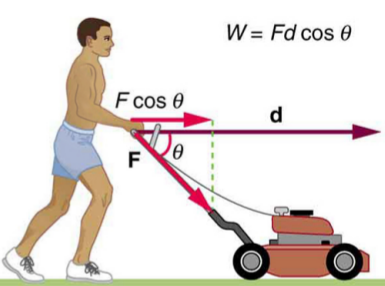
\includegraphics[width=\textwidth]{figures/lawn1.png}
\caption{}
\end{subfigure}
\begin{subfigure}{0.135\textwidth}
\centering
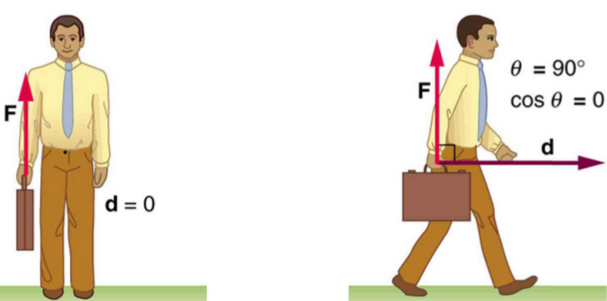
\includegraphics[width=\textwidth,trim=0cm 0cm 15cm 0cm,clip=true]{figures/lawn2.png}
\caption{}
\end{subfigure}
\begin{subfigure}{0.2\textwidth}
\centering
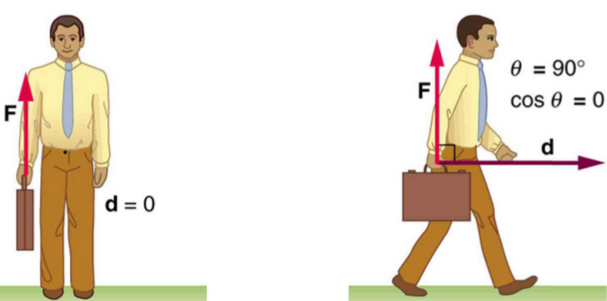
\includegraphics[width=\textwidth,trim=12cm 0cm 0cm 0cm,clip=true]{figures/lawn2.png}
\caption{}
\end{subfigure}
\begin{subfigure}{0.45\textwidth}
\centering
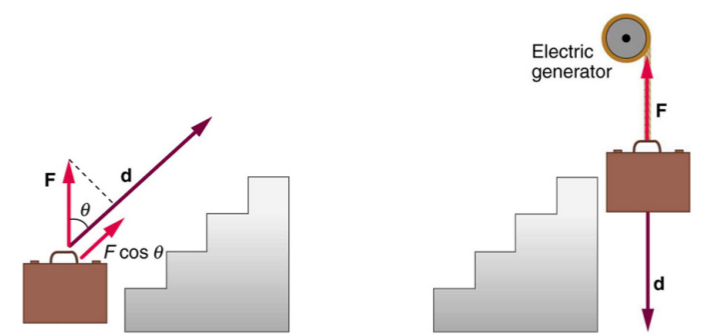
\includegraphics[width=\textwidth]{figures/lawn3.png}
\caption{}
\end{subfigure}
\caption{\label{fig:workvisual}\small (a) General case of work (b) No work, $d=0$ (c) No work, $\vec{F}\cdot\vec{d}=0$ (d) Positive work, then negative work}
\end{figure}
\end{frame}

\begin{frame}{Definition of Work}
Work has the unit of the \textit{Joule}, which is denoted \\ \textbf{1 J = 1 N m, or 1 kg m$^2$ s$^{-1}$.} \\  \vspace{1cm}
\small
\alert{Potential Paper Topic:}\\
\textit{Extra credit opportunity}: \textbf{Do you like beer}?  Write a 10-page paper on the on the scientific challenge faced by James Prescott Joule, who began to formulate the modern view of energy in the 19th century, contrary to \textit{caloric theory}.
\end{frame}

\begin{frame}{Definition of Work}
\begin{figure}
\centering
\begin{subfigure}{0.12\textwidth}
\centering
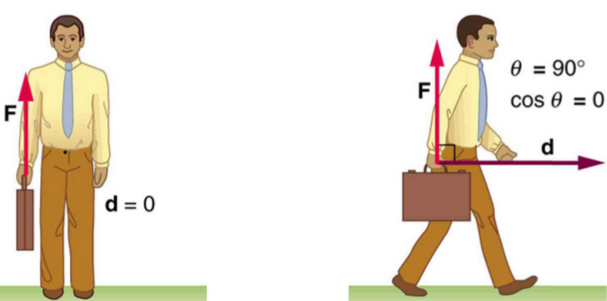
\includegraphics[width=\textwidth,trim=0cm 0cm 15cm 0cm,clip=true]{figures/lawn2.png}
\caption{}
\end{subfigure}
\begin{subfigure}{0.18\textwidth}
\centering
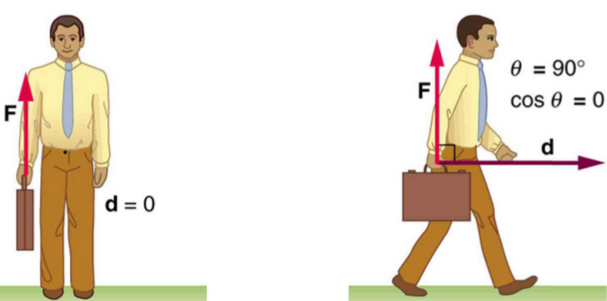
\includegraphics[width=\textwidth,trim=12cm 0cm 0cm 0cm,clip=true]{figures/lawn2.png}
\caption{}
\end{subfigure}
\begin{subfigure}{0.43\textwidth}
\centering
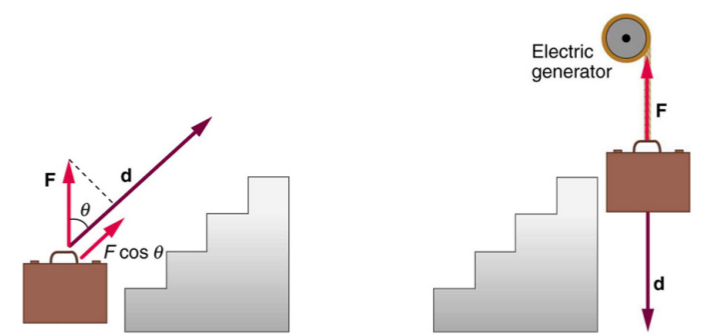
\includegraphics[width=\textwidth]{figures/lawn3.png}
\caption{}
\end{subfigure}
\caption{\label{fig:workvisual2} Different cases involving work.}
\end{figure}
\small
Rank the work done \textit{on the briefcase by F} from greatest to least.
\begin{itemize}
\item A: Case C (left) > Case A = Case B > Case C (right)
\item B: Case C (right) > Case A = Case B > Case C (left)
\item C: Case C (left) > Case A > Case B > Case C (right)
\item D: Case C (left) > Case B > Case A > Case C (right)
\end{itemize}
\end{frame}

\begin{frame}{Definition of Work}
\begin{figure}
\centering
\begin{subfigure}{0.3\textwidth}
\centering
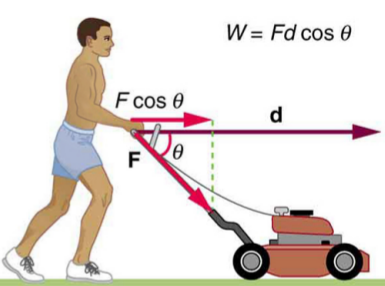
\includegraphics[width=\textwidth]{figures/lawn1.png}
\caption{}
\end{subfigure}
\begin{subfigure}{0.135\textwidth}
\centering
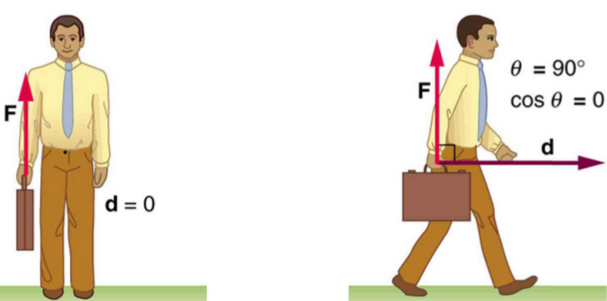
\includegraphics[width=\textwidth,trim=0cm 0cm 15cm 0cm,clip=true]{figures/lawn2.png}
\caption{}
\end{subfigure}
\begin{subfigure}{0.2\textwidth}
\centering
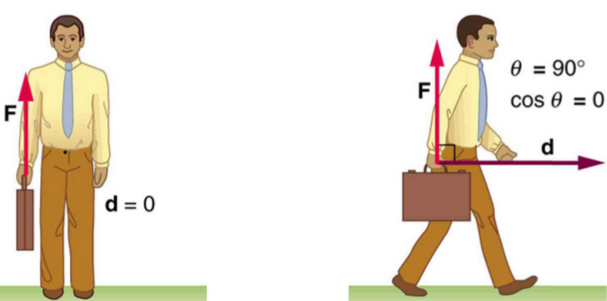
\includegraphics[width=\textwidth,trim=12cm 0cm 0cm 0cm,clip=true]{figures/lawn2.png}
\caption{}
\end{subfigure}
\caption{\label{fig:workvisual3} Different cases involving work.}
\end{figure}
\small
Rank the work \textit{on the mower/briefcase by F} from greatest to least.
\begin{itemize}
\item A: Case C > Case B > Case A
\item B: Case B = Case C > Case A
\item C: Case A > Case B = Case C
\item D: Case A = Case B = Case C
\end{itemize}
\end{frame}

\begin{frame}{Definition of Work}
\begin{figure}
\centering
\begin{subfigure}{0.3\textwidth}
\centering
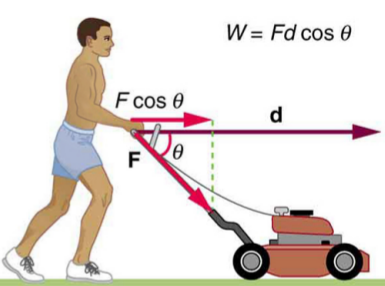
\includegraphics[width=\textwidth]{figures/lawn1.png}
\caption{}
\end{subfigure}
\begin{subfigure}{0.2\textwidth}
\centering
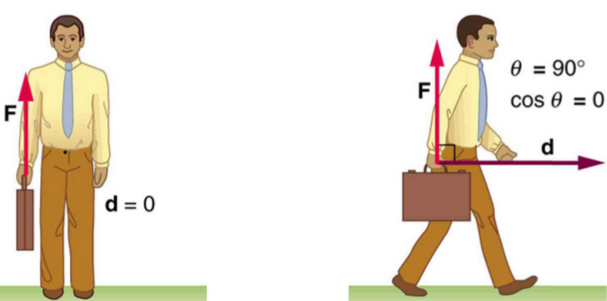
\includegraphics[width=\textwidth,trim=12cm 0cm 0cm 0cm,clip=true]{figures/lawn2.png}
\caption{}
\end{subfigure}
\caption{\label{fig:workvisual4} Different cases involving work.}
\end{figure}
\small
Which changes would \textit{increase} the work in both Case A and Case B?
\begin{itemize}
\item A: Case A: decrease $\theta$, Case B: decrease $\theta$.
\item B: Case A: increase $\theta$, Case B: decrease $\theta$.
\item C: Case A: decrease $\theta$, Case B: increase $\theta$.
\item D: Case A: increase $\theta$, Case B: increase $\theta$.
\end{itemize}
\end{frame}

\begin{frame}{Definition of Work}
Suppose a system is displaced by $\vec{d} = 2\hat{i}-3\hat{j}$ m by a force $\vec{F} = -3\hat{i}+5\hat{j}$ N.  What is the work done on the system by $\vec{F}$?
\begin{itemize}
\item A: 21 J
\item B: -21 J
\item C: 15 J
\item D: -15 J
\end{itemize}
\end{frame}

\begin{frame}{Definition of Work}
Suppose a system is displaced by $\vec{d} = 2\hat{i}-3\hat{j}$ m \textit{against} a force $\vec{F} = -3\hat{i}+5\hat{j}$ N.  What is the work done on the system by $\vec{F}$, if the system moves at constant velocity?
\begin{itemize}
\item A: 21 J
\item B: -21 J
\item C: 15 J
\item D: -15 J
\end{itemize}
\end{frame}

\begin{frame}{Definition of Work}
As we will see, work is a form of \textit{energy}.  There are other units of energy which apply to different \textit{energy scales}.  A human being requires about 2000 kcal of food energy per day.  If 1 kcal equals 1000 calories, and 1 calorie equals 4.184 J, how many Joules of energy does one human require per day?
\begin{itemize}
\item A: 1 kJ (a thousand Joules)
\item B: 10 kJ (ten thousand Joules)
\item C: 1 MJ (a million Joules)
\item D: 10 MJ (ten million Joules) 
\end{itemize}
\end{frame}

\begin{frame}{Definition of Work}
Calculate the mass of an object displaced 1 meter ($d = 1\hat{j}$) \textit{against} gravity, $F = -mg\hat{j}$, if the work done was equal to 10 MJ.
\begin{itemize}
\item A: 1000 kg
\item B: 10,000 kg
\item C: 100,000 kg
\item D: 1,000,000 kg
\end{itemize}
\textit{Our bodies burn a lot of energy...we will return to this!}
\end{frame}

\begin{frame}{Definition of Work}
\small
More units of energy:
\begin{table}
\centering
\begin{tabular}{c | c | c}
\alert{Unit Name} & \alert{Definition} & \alert{Value} \\ \hline
electron-volt (eV) & energy of 1 e$^{-}$ through 1 V & $1.60\times 10^{-19}$ J \\ \hline
1 Rydberg (Rd) & ionize 1 hydrogen atom & $21.8\times 10^{-19}$ J \\ \hline
\textbf{Joule} & \textbf{1 N$\cdot$m} & \textbf{1.0 J} \\ \hline
foot-pound & 1 ft$\cdot$lb & 1.36 J \\ \hline
calorie & Raise 1 gram of water 1$^{\circ}$ C & 4.184 J \\ \hline
British Thermal Unit & Raise 1 lb of ice to boil ($^{\circ}$F) & 1054.3 J \\ \hline
food calorie (kcal) & 1000 calories & 4184 J \\ \hline
kilowatt hours & 1 kilowatt system for 1 hr & $3.6\times 10^6$ J \\ \hline
gasoline galon equiv. & burning a galon of gas & $\approx 120 \times 10^6$ J \\ \hline
$E = mc^2$, 1 mole of H$^{+}$ & Rest mass (fusion/fission) & $9 \times 10^{13}$ J \\ \hline
\end{tabular}
\end{table}
\end{frame}

\begin{frame}{Definition of Work}
\begin{figure}
\centering
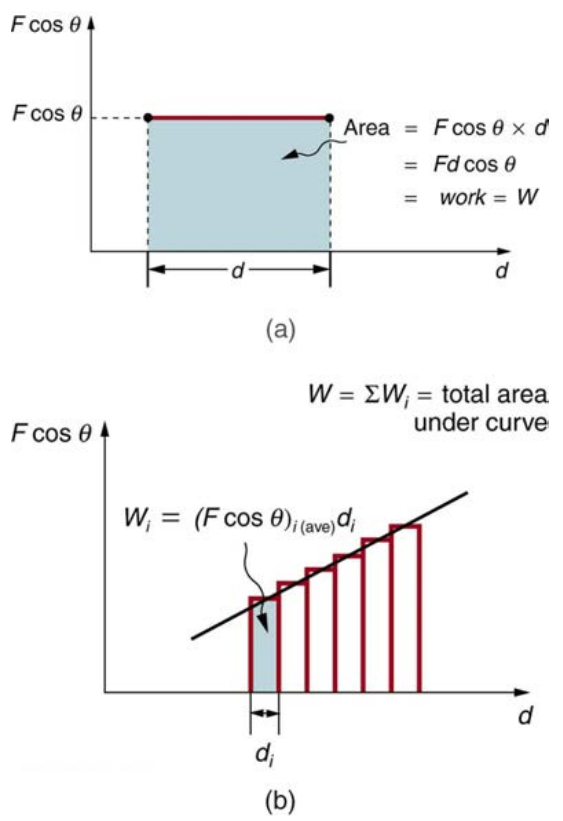
\includegraphics[width=0.4\textwidth]{figures/area.png}
\caption{\label{fig:area} Generally, work is the area under a curve of force applied versus displacement.}
\end{figure}
\end{frame}

\begin{frame}{Definition of Work}
Suppose a 100 kg system is displaced 5 m through a region with kinetic friction coefficient of 0.02, and then displaced by 10 m through a region with kinetic friction coefficient 0.01.  What is the work done on the system?
\begin{itemize}
\item A: 10 J
\item B: 20 J
\item C: 100 J
\item D: 200 J
\end{itemize}
\end{frame}

\begin{frame}{Definition of Work}
Notice from this problem, that we had to discover an equation: $W = \mu m g d$.  This is the work done against friction when friction is the net force, and $d$ is the displacement. \\ \vspace{1cm}
\textbf{Work against friction net force:}
\begin{equation}
W = -\mu m g d
\end{equation}
\textbf{Note:} \textit{Why the minus sign?} The force of friction is oriented opposite the direction of the displacement.  Remember: $W = \vec{F}\cdot\vec{d}$.
\end{frame}

\begin{frame}{Definition of Work}
Suppose the driver of a vehicle of mass $m$ traveling at speed $v$ hits the brakes, and the car slides to a stop after a distance $d$.  What is the net force on the vehicle as it slides to a stop?
\begin{itemize}
\item A: $F = ma$
\item B: $F = mgd$
\item C: $F = \mu m g d$
\item D: $F = \mu m g$
\end{itemize}
\end{frame}

\begin{frame}{Definition of Work}
For the same scenario, derive an expression for the distance $d$, if the initial speed is $v$ and the final speed is zero.  Use one of the kinematic equations.
\begin{itemize}
\item A: $d = \frac{1}{2\mu g} v^2$
\item B: $d = vt$
\item C: $d = \frac{1}{2}at^2$
\item D: $d = \frac{1}{2\mu g} v$
\end{itemize}
\end{frame}

\begin{frame}{Definition of Work}
Substitute the expression derived for $d$ into the expression for the work done on the car to bring it to a stop ($W = -\mu m g d$).  What is the result?
\begin{itemize}
\item A: $W = -\frac{1}{2} m v^2$
\item B: $W = mv$
\item C: $W = mv^2$
\item D: $W = \frac{1}{2} m v^2$
\end{itemize}
\end{frame}

\begin{frame}{Definition of Work}
The answer is that the vehicle loses an energy equal to $-\frac{1}{2}mv^2$.  In general, the expression $KE = \frac{1}{2}mv^2$ is denoted the \textit{kinetic energy}.  In the problem, the work \textit{took away} the kinetic energy, or, the energy was lost to the work done by friction. \\ \vspace{1cm}
\textbf{Potential energy:} energy stored that may later be converted back to kinetic energy.
\end{frame}

\begin{frame}{Definition of Work}
\textbf{Potential energy:}
Consider the work done by gravity if an object is lifted a distance $\Delta y$ at constant.  Apply the definition of work:
\begin{equation}
W_g = \vec{F}_g \cdot \Delta \vec{y} = -mg \hat{j} \cdot \Delta \vec{y} = -mg\Delta y
\end{equation}
By Newton's Third Law, if the work done \textit{by} gravity is $-mg\Delta y$, then the work done \textit{against} gravity is
\begin{equation}
U = m g \Delta y
\end{equation}
We will call this energy \textit{gravitational potential energy.}
\end{frame}

\section{Kinetic Energy and the Work-Energy Theorem}

\begin{frame}{Kinetic energy and the work-energy theorem}
To obtain this theorem, we combine two concepts: \alert{\textbf{Newton's 2nd Law}} and \alert{\textbf{the definition of work}}.  Start with the definition of work, and substitute for the force using Newton's 2nd Law:
\begin{align}
W_{\rm Net} &= \vec{F}_{\rm Net} \cdot \vec{d} \\
W_{\rm Net} &= m\vec{a}_{\rm Net} \cdot \vec{d} \\
W_{\rm Net} &= m\left(\frac{v^2-v_{\rm 0}^2}{2d}\right) d \label{eq:this} \\
W_{\rm Net} &= \frac{1}{2}mv^2 - \frac{1}{2}mv_{\rm 0}^2 \label{eq:this2}
\end{align}
In Eq. \ref{eq:this}, we assume that the force and displacement are aligned, but this can be done infinitesimally and is therefore not a special case. The two terms in Eq. \ref{eq:this2} have units of Joules.
\end{frame}

\begin{frame}{Kinetic Energy and the Work-Energy Theorem}
\begin{tcolorbox}[colback=white,colframe=red!40!blue,title=The Work-Energy Theorem]
\small
\alert{
Let the \textit{kinetic energy} of a system with mass $m$ be defined to be $KE = \frac{1}{2}mv^2$.  The work done on a system is equal to the change in kinetic energy:
\begin{equation}
W = KE_{\rm f} - KE_{\rm i} = \Delta KE
\end{equation}
}
\end{tcolorbox}
\end{frame}

\section{Lab Activity: Work-Energy Theorem, and the Conservation of Energy}

\begin{frame}{Gravitational Potential Energy}
\textbf{The famous roller coaster problem}: Suppose a roller coaster has a circular loop with radius $R$, and the cars begin on a hill of height $y_{\rm 1}$.  Since work has been performed on the cars to get them that high, they have energy $W = mgy_{\rm 1}$ (they have mass $m$).  When that gravitational potential energy is converted to kinetic, the cars are propelled through the loop.  What is the ratio of $y_{\rm 1}$ to $R$? 
\begin{columns}[T]
\begin{column}{0.5\textwidth}
\begin{itemize}
\item A: $y_{\rm 1} = \frac{1}{2}R$
\item B: $y_{\rm 1} = R$
\item C: $y_{\rm 1} = \frac{3}{2}R$
\item D: $y_{\rm 1} = \frac{5}{2}R$
\end{itemize}
\end{column}
\begin{column}{0.5\textwidth}
\begin{figure}
\centering
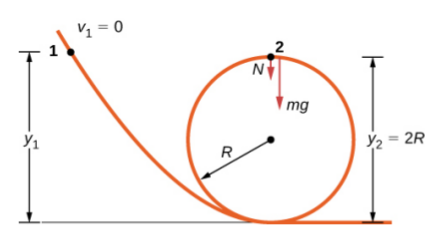
\includegraphics[width=\textwidth]{figures/loop.png}
\end{figure}
\end{column}
\end{columns}
\end{frame}

\begin{frame}{Gravitational Potential Energy and Work-Energy Theorem}
\small
\begin{columns}[T]
\begin{column}{0.33\textwidth}
\textbf{Materials (5 min)}:
\begin{itemize}
\item Pipe liner
\item A ball bearing
\item Scissors
\item Tape
\item Ruler
\end{itemize}
\end{column}
\begin{column}{0.33\textwidth}
\textbf{Build (10 min)}:
\begin{itemize}
\item Cut pipe liner in half, lengthwise
\item Shape the pipe liner into the shape on prior slide
\item Use tape to fix in place
\end{itemize}
\end{column}
\begin{column}{0.33\textwidth}
\textbf{Measure (15 minutes)}:
\begin{itemize}
\item Measure the initial height required to traverse loop
\item Compare to loop radius
\item Report the radius and ten initial height measurements
\end{itemize}
\end{column}
\end{columns}
\alert{\textbf{Bonus}: \textit{Two loops?}}
\end{frame}

\begin{frame}{Gravitational Potential Energy and Work-Energy Theorem}
\small
\begin{columns}[T]
\begin{column}{0.5\textwidth}
\textbf{Measure}:
\begin{itemize}
\item Measure the initial height required to traverse loop
\item Compare to loop radius
\item Report the radius and trials of initial height measurements
\end{itemize}
\end{column}
\begin{column}{0.5\textwidth}
\textbf{Compare answers to class}:
\begin{itemize}
\item Find the average of all initial height trials, and compute the standard deviation
\item Give average and standard deviation, both divided by the loop radius, to professor
\item Professor will combine data
\item \textbf{Discussion of results, and possible sources of error}
\end{itemize}
\end{column}
\end{columns}
\end{frame}

\begin{frame}{Kinetic Energy and the Work-Energy Theorem}
First, a problem with kinetic energy.  What is the kinetic energy of a baseball that weighs 150 grams that is pitched at 140 km/hour?  (Convert to meters per second and kilograms).
\begin{itemize}
\item A: 75 J
\item B: 50 J
\item C: 25 J
\item D: 5 J
\end{itemize}
\end{frame}

\begin{frame}{Kinetic Energy and the Work-Energy Theorem}
A \textit{cosmic ray} is an ultra-high energy proton that can be detected with kinetic energies up to $10^{19}$ eV.  An eV (electron-Volt) is a strange unit of energy used in particle physics, and 1 eV = $1.6 \times 10^{-19}$ eV.  If a cosmic ray has $10^{19}$ eV, how much energy is this in Joules?
\begin{itemize}
\item A: 0.16 J
\item B: 1.6 J
\item C: 16 J
\item D: 160 J
\end{itemize}
\end{frame}

\begin{frame}{Kinetic Energy and the Work-Energy Theorem}
Now that we have familiarity with kinetic energy, let's look at \textit{gravitational potential energy}.
\begin{figure}
\centering
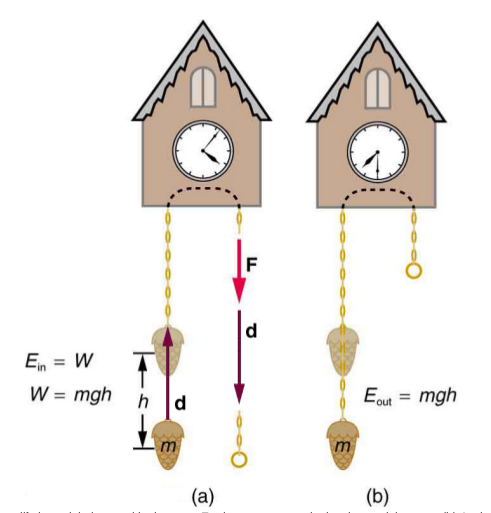
\includegraphics[width=0.4\textwidth]{figures/clock.png}
\caption{\label{fig:clock} Work done against gravity ($m g h$) is stored as \textit{potential energy}, to be converted to kinetic energy later.}
\end{figure}
\end{frame}

\begin{frame}{Kinetic Energy and the Work-Energy Theorem}
The work done to stretch a spring with spring constant $k$ by a displacement $x$ is $W = \frac{1}{2}kx^2$.  (\textit{Why?  We will answer this below}).  Suppose gravity pulls the weight on the clock in Fig. \ref{fig:clock}, such that it compresses an internal spring with spring constant $k$ by $x$.  If all of the gravitational potential energy is converted to potential energy in the spring, what is the expression for the displacement $x$? \\ \vspace{1cm}
\textbf{Solve this by groups on boards}.
\end{frame}

\begin{frame}{Kinetic Energy and the Work-Energy Theorem}
When the clock strikes the hour, it launches a wooden cuckoo horizontally out the front, using the stored potential energy in the spring.  What is the velocity of the wooden cuckoo?  (The mass of the weight is 100 grams, $g = 10$ m/s$^2$, $h = 20$ cm, and $k = 10$ N/m).\\ \vspace{1cm}
\textbf{Solve this by groups on boards}.
\end{frame}

\begin{frame}{Kinetic Energy and the Work-Energy Theorem}
\textit{Gravitational potential energy} can also be converted to kinetic energy by the work energy theorem:
\begin{figure}
\centering
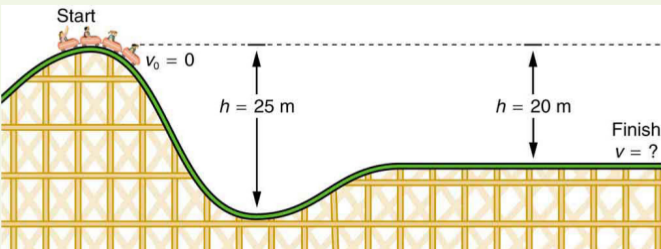
\includegraphics[width=0.6\textwidth,trim=0.25cm 0cm 0cm 0.25cm,clip=true]{figures/roller.png}
\caption{\label{fig:roller} The initial gravitational potential energy is converted to kinetic energy, give the riders speed.}
\end{figure}
\end{frame}

\begin{frame}{Kinetic Energy and the Work-Energy Theorem}
Suppose the difference in height from beginning to end is $20$ m.  What is the final speed, $v$? \\ \vspace{1cm}
\begin{itemize}
\item A: 2 m/s
\item B: 10 m/s
\item C: 20 m/s
\item D: 100 m/s
\end{itemize}
\end{frame}

\section{Gravitational Potential Energy and Conservative Forces}

\begin{frame}{Graviational potential energy and conservative forces}
Gravity is an example of a \textit{conservative force}: the work done against it does not depend on the path of the system through it.  This is true of gravity.  \textbf{The work done to move a system through a gravity field does not depend on the path taken.} \\ \vspace{1cm}
\begin{columns}[T]
\begin{column}{0.3\textwidth}
\centering
\underline{Force}
\begin{itemize}
\item $\vec{F} = -mg\hat{j}$
\item $\vec{F} = -kx\hat{i}$
\item $\vec{F} = -\left(\frac{mg}{L}\right)x\hat{i}$
\end{itemize}
\end{column}
\begin{column}{0.7\textwidth}
\centering
\underline{Potential Energy}
\begin{itemize}
\item $U(y) = mgy$
\item $U(x) = \frac{1}{2}kx^2$
\item $U(x) = mgL(1-\cos\theta) \approx \frac{mg}{2L}x^2$
\end{itemize}
\end{column}
\end{columns} \vspace{0.5cm}
\small
\textbf{If there is a potential energy associated with a force, it is conservative.}  Can you see the relationship between the potentials and the forces?
\end{frame}

\section{Power}

\begin{frame}{Power}
Power is simple once we understand work and energy.  Let $W$ be the work done on a system, increasing the kinetic energy of the system.  The change in kinetic energy $W$ divided by the time required for that change to take place, $T$, is the \alert{\textit{power}}:
\begin{equation}
\boxed{
P = \frac{W}{T}
}
\end{equation}
In terms of calculus, the \textit{area under a curve} of \textit{power versus time} is the work done on a system.  The units of power are Joules per second, or Watts.
\end{frame}

\begin{frame}{Power}
Suppose a cyclist is racing in Le Tour de France, and climbs a section of road where the vertical displacement is 100 m.  The mass of the bicycle is negligible, and the mass of the cyclist is 60 kg ($g = 10$ m/s$^2$).  If the climb takes 100 seconds, what power is the cyclist expending?
\begin{itemize}
\item A: 200 Watts
\item B: 400 Watts
\item C: 600 Watts
\item D: 1000 Watts
\end{itemize}
\end{frame}

\begin{frame}{Power}
Recall that $W = \Delta KE$, that is, the work-energy theorem, plus any stored potential energy (conservation of energy).  Suppose a 50 kg athelete is training by running up a hill.  Her initial speed is zero, but her final speed is 2 m/s.  The hill is a vertical displacement of 10 meters.  If she makes it up the hill in 10 seconds, how much power is she producing?
\begin{itemize}
\item A: 510 Watts
\item B: 205 Watts
\item C: 50 Watts
\item D: 1050 Watts
\end{itemize}
\end{frame}

\begin{frame}{Power}
Suppose your monthly electricity bill is \$30.00.  What is your electrical energy consumption, if the price of electricity is \$0.20 per kilowatt-hour?
\begin{itemize}
\item A: 105 Watts
\item B: 208 Watts
\item C: 505 Watts
\item D: 1000 Watts
\end{itemize}
\end{frame}

\begin{frame}{Power}
The human body stores excess energy, burns heat, and does work:
\begin{figure}
\centering
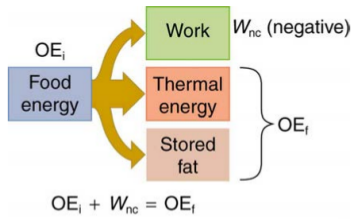
\includegraphics[width=0.5\textwidth]{figures/body.png}
\end{figure}
\end{frame}

\begin{frame}{Power}
The human body stores excess energy, burns heat, and does work:
\begin{figure}
\centering
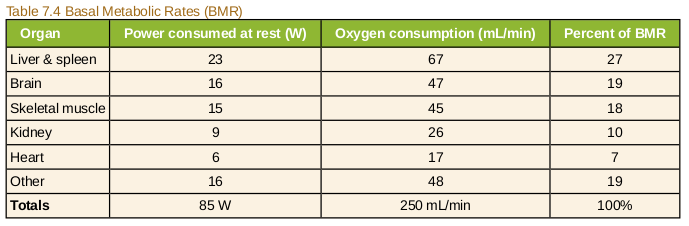
\includegraphics[width=0.8\textwidth]{figures/body2.png}
\end{figure}
The body burns some energy at a the given wattages, whether we do \textit{useful} work or not.  To calculate weight gain, this \textit{base metabolic rate} must be taken into account.
\end{frame}

\begin{frame}{Power}
Various activities:
\begin{figure}
\centering
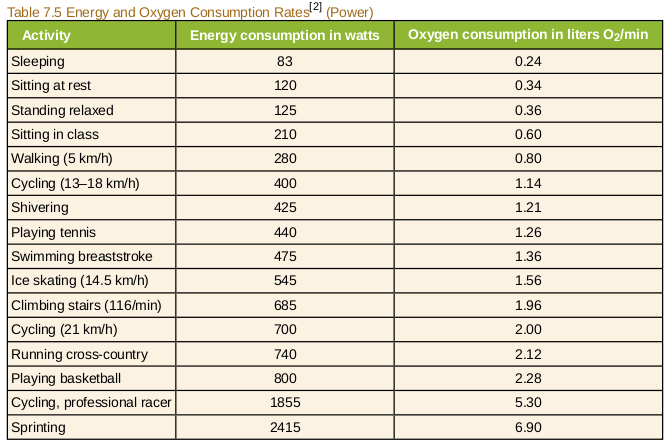
\includegraphics[width=0.8\textwidth]{figures/body3.png}
\end{figure}
\end{frame}

\begin{frame}{Power}
\textbf{Unit-concluding activity}: choose an activity from the prior table, and choose an interval of time to do it.  Knowing how much power it takes to operate the human body, derive the number of kcal (Calories) required to do that activity.
\end{frame}

\section{Conclusion}

\begin{frame}{Week 7 Summary}
\begin{enumerate}
\item \alert{Work} has a scientifically precise definition
\item Kinetic Energy and the \alert{Work-Energy Theorem}
\item Gravitational potential energy
\item Definition of a \textbf{conservative force} and potential energy
\item Power and the human body
\end{enumerate}
\end{frame}

\end{document}
